\begin{surferPage}[Labs-Septik]{Eine Septik mit 99 Singularitäten}
   Oliver Labs konstruierte im Rahmen seiner Dissertation in Mainz 2004 eine
    Fläche vom Grad $7$ (Septik) mit $99$ Singularitäten: derzeit Weltrekord! 
    Bisher ist aber kein Grund bekannt, warum es nicht sogar eine Septik mit
    $104$ Singulariäten geben könnte!  
    Labs' Fläche hat die Symmetrie eines regelmäßigen $7$-Ecks.
    Man sieht dies recht gut, wenn man die Fläche von ``oben'' betrachtet:
    \vspace*{-0.3em}
    \begin{center}
      \begin{tabular}{c@{\qquad}c}
        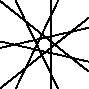
\includegraphics[height=1.5cm]{./../../common/images/labsseptic1.pdf}
        &
        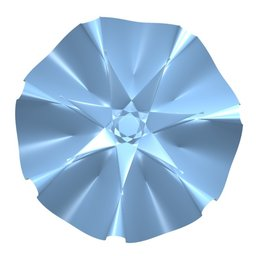
\includegraphics[height=1.5cm]{./../../common/images/labs_septic_von_oben}
      \end{tabular}
    \end{center}
    \vspace*{-0.3em}
    Zur Suche nach der Fläche hat O.\ Labs das Computeralgebraprogramm
    {\sc Singular} (Universit\"at Kaiserslautern) benutzt, dessen besondere Stärke in
    Anwendungen auf 
    algebraischer Geometrie und Singularitäten liegt.

    Dabei hat er ausgenutzt, dass man in endlichen
    Zahlensystemen rechnen kann. Von der Uhr kennen wir dies: 24 Uhr
    entspricht 0 Uhr, 24 Uhr $+$ 1 Stunde ist nicht 25 Uhr, sondern 1
    Uhr.
\end{surferPage}
